\documentclass[a4paper,10pt]{article}
\usepackage[utf8]{inputenc}
\usepackage{listings}
\usepackage{color}
\usepackage{url}
\usepackage{hyperref}
\usepackage{graphicx}

\definecolor{grey}{rgb}{0.9,0.9,0.9}

\lstset{
language=Python,
basicstyle=\footnotesize\fontfamily{pcr},
backgroundcolor=\color{grey},
numbers=left,
numberstyle=\tiny,
numbersep=5pt,
showstringspaces=false,
tabsize=3,
breaklines=true
}

\setlength{\parindent}{0pt} 

%opening
\title{INFO-F-413 : Problème des Secrétaires}
\author{Thomas Chapeaux}

\begin{document}
\sloppy
\maketitle

\section{Présentation}

Le problème des Secrétaires\footnote{Ref. [1]} est un exemple de problème d'arrêt optimal. On imagine une situation où l'on veut engager
le meilleur candidat parmis
\begin{math}n\end{math}
(selon une métrique donnée et qui ne crée pas d'égalités). Les candidats sont évalués un à un dans un ordre aléatoire et on doit choisir si on engage un candidat
avant d'évaluer le suivant. Le problème consiste à trouver une méthode qui nous permettra d'engager le meilleur candidat avec
la plus grande probabilité possible.\\

La stratégie étudiée ici consiste à évaluer les
\begin{math}m = \frac{n}{e}\end{math}
premiers candidats et à tous les rejeter mais en retenant la valeur
\begin{math}s\end{math}
du meilleur score observé. Ensuite, on évalue les
\begin{math}n-m\end{math}
candidats restants et on engage le premier candidat dont le score est supérieur à
\begin{math}s\end{math}.\\

\section{Analyse théorique}
Cette analyse théorique se base sur l'exercice 2.32 de l'ouvrage de référence du cours\footnote{Ref. [2]}.
\subsection{Probabilité d'engager le meilleur candidat}
(Ce calcul se base sur celui détaillé sur la page Wikipédia du problème\footnote{Ref. [3]}\\

Notons
\begin{math}Pr(E_i)\end{math}
la probabilité que l'employé
\begin{math}i\end{math}
soit le meilleur candidat
(\begin{math}best_i\end{math})
et qu'il soit sélectionné
(\begin{math}choix_i\end{math})
, on a donc (selon la définition de variable aléatoires indépendantes) :\\

\begin{math}\;\;Pr(E_i) = Pr(best_i \cap choix_i) = Pr(choix_i\ |\ best_i) * Pr(best_i)\end{math}\\

Si
\begin{math}i < m\end{math},
on a
\begin{math}Pr(choix_i) = 0\end{math}
indépendamment de
\begin{math}best_i\end{math}.
On s'intéresse donc seulement aux
\begin{math}i > m\end{math}.
De plus, comme il n'y a aucune relation entre l'ordre des candidats et leur score, on a
\begin{math}\;\;Pr(best_i) = \frac{1}{n}\end{math}.\\

Sachant que
\begin{math}i > m\end{math}
est le meilleur candidat, il sera sélectionné si aucun candidat dont le score est meilleur que celui des
\begin{math}m\end{math}
premiers ne se trouve entre
\begin{math}m\end{math}
et
\begin{math}i\end{math}.
Autrement dit, si le meilleur candidat parmis les
\begin{math}i - 1\end{math}
premiers se trouve parmis les
\begin{math}m\end{math}
premiers. Et comme l'ordre de passage est aléatoire, ceci arrive avec une probabilité
\begin{math}\frac{m}{i-1}\end{math}.
On a donc :\\

\begin{math}\;\;Pr(E_i) = \frac{m}{i-1} * \frac{1}{n}\ \forall i > m\end{math}\\

Sachant cela, la probabilité que l'on engage effectivement le meilleur candidat vaut :\\

\begin{math}\;\;Pr(E) = \sum_{i=0}^n Pr(E_i) = 0 + \sum_{i=m+1}^n \frac{m}{i-1} * \frac{1}{n} = \frac{m}{n} \sum_{i=m+1}^{n} \frac{1}{i-1}\end{math}

\subsection{Calcul de la somme}

En effectuant le changement de variable
\begin{math}i = i'+1\end{math},
on trouve :\\

\begin{math}\;\;Pr(E) = \frac{m}{n} \sum_{i'=m}^{n-1} \frac{1}{i'}\end{math}\\

La somme de cette expression peut se représenter de la manière suivante sur la courbe
\begin{math}f(x) = \frac{1}{x}\end{math}:\\

[graphique 1]\\

Ici, chaque terme de la somme est d'abord représenté par un rectangle jaune de largeur 1 et de longueur
\begin{math}\frac{1}{i}\end{math}
placé à droite de la valeur
\begin{math}i\end{math} correspondante. Ceci permet de voir clairement que la somme est strictement supérieure à
\begin{math}\int_m^n \frac{1}{x} dx = ln(m) - ln(n)\end{math}\\

Ensuite, en dessinant les rectangles vers la gauche (en hachuré), on voit clairement que la somme est également strictement
inférieure à, cette fois, 
\begin{math}\int_{m-1}^{n-1} \frac{1}{x} dx = ln(m-1) - ln(n-1)\end{math}\\

On a donc bien la propriété recherchée :\\

\begin{math}\;\;\frac{m}{n} (ln(n) - ln(m)) \leq Pr(E) \leq \frac{m}{n} (ln(n-1) - ln(m-1))\end{math}\\

\subsection{Calcul de la valeur optimale de m}

On veut trouver la valeur de 
\begin{math}m\end{math}
qui nous donne la meilleure probabilité de choisir le meilleur candidat. Ceci revient à calculer le maximum de\\

\begin{math}\;\;f(m) = \frac{m}{n} (ln(n) - ln(m))\end{math}\\

Ceci se fait en annulant la dérivée :\\

\begin{math}\;\;f'(m) = \frac{ln(n) - ln(m) - 1}{n}\end{math}\\

\begin{math}\;\;f'(m) = 0 \Leftrightarrow ln(m) = ln(n) - 1\Leftrightarrow e^{ln(m)} = e^{ln(n) - 1}\Leftrightarrow m = \frac{n}{e}\end{math}\\

On peut donc calculer la borne inférieure de probabilité de succès trouvée précédemment\\

\begin{math}\;\; Pr(E) \geq \frac{m}{n} (ln(n) - ln(m))\end{math}\\

\begin{math}\;\; m = \frac{n}{e} \Rightarrow Pr(E) \geq \frac{1}{n} \frac{n}{e}(ln(n) - ln(\frac{n}{e}))
= \frac{1}{e} (ln(n) - ln(n) + 1) = \frac{1}{e}\end{math}\\

\section{Discussion}
Afin de vérifier les résultats précédents, une implémentation en Python du problème et de la solution discutée a été effectuée.
Le code de celle-ci se trouve en annexe. L'implémentation effectuait une série de 1000 tests sur un ensemble de 100 candidats.

\subsection{Probabilité de réussite}
Pour
\begin{math}n = 100\end{math},
on a
\begin{math}m = \frac{n}{e} \approx 37\end{math}.
Avec cette valeur, notre implémentation trouve le meilleur candidat avec
une probabilité
\begin{math}P = 0.385 > \frac{1}{e} \approx 0.368\end{math}.
Ceci correspond donc à l'analyse qui avait été faite.

\subsection{Valeur de m}
On a vu que
\begin{math}m = \frac{n}{e} \approx 37\end{math}
était la valeur avec la plus grande probabilité de succès pour notre cas
(\begin{math}n = 100\end{math}).
Le graphe suivant montre l'évolution du taux de réussite en fonction de
\begin{math}m\end{math}. 
La valeur optimale théorique a été indiquée en bleu.

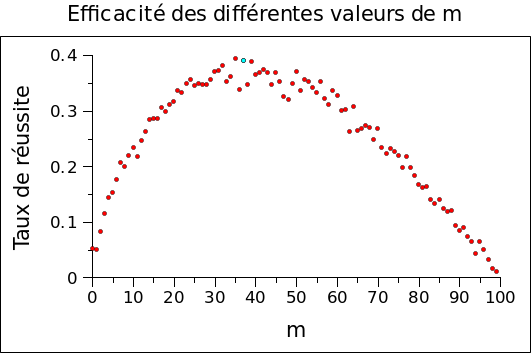
\includegraphics[scale=0.5]{../success_m_graph.png}\\

On voit clairement que
\begin{math}m = 37\end{math}
est très proche du maximum.\\

Cette courbe confirme également notre analyse théorique, où on avait trouvé que la relation entre
\begin{math}m\end{math}
et
\begin{math}Pr(E)\end{math}
était bornée par :\\

\begin{math}\;\;\frac{m}{n} (ln(n) - ln(m)) \leq Pr(E) \leq \frac{m}{n} (ln(n-1) - ln(m-1))\end{math}\\

Le graphe expérimental trouvé précédemment coincide avec le graphe de ces deux fonctions :

\includegraphics[scale=0.75]{../success_m_graph_the.png}\\
(Source : Wolfram Alpha\footnote{Ref. [4]}

\section{Références}
\begin{itemize}
  \item {[}1] \url{http://en.wikipedia.org/wiki/Secretary_problem}, visité le 21 Octobre 2012
  \item {[}2] “Probability and Computing”, by M. Mitzenmacher and E. Upfal, Cambridge
  \item {[}3] \url{http://en.wikipedia.org/wiki/Secretary_problem#Deriving_the_optimal_policy}, visité le 21 Octobre 2012
  \item {[}4] \url{www.wolframalpha.com} Requète exacte : \url{http://is.gd/JstESE}
\end{itemize}
\section{Annexes}

\subsection{Génération de l'ordre de passage}

\subsection{Améliorations possibles}

\begin{itemize}
  \item Optimisation du temps de calcul pour la génération de l'ordre de passage
  \item Analyse plus fine des résultats
\end{itemize}


\subsection{Code source complet}
Le code a normalement été fourni avec le présent rapport. Il est aussi disponible sur GitHub :\\
\url{https://github.com/BafAltom/info-f413-secretary-problem}
\fontfamily{pcr}
\lstinputlisting[language=Python]{../main.py}
\fontfamily{}


\end{document}
